\documentclass[10pt, letterpaper]{article}

\usepackage{graphicx}

% Packages:
\usepackage[
    ignoreheadfoot, % set margins without considering header and footer
    top=2 cm, % seperation between body and page edge from the top
    bottom=2 cm, % seperation between body and page edge from the bottom
    left=2 cm, % seperation between body and page edge from the left
    right=2 cm, % seperation between body and page edge from the right
    footskip=1.0 cm, % seperation between body and footer
    % showframe % for debugging 
]{geometry} % for adjusting page geometry
\usepackage{titlesec} % for customizing section titles
\usepackage{tabularx} % for making tables with fixed width columns
\usepackage{array} % tabularx requires this
\usepackage[dvipsnames]{xcolor} % for coloring text
\definecolor{primaryColor}{RGB}{0, 0, 0} % define primary color
\usepackage{enumitem} % for customizing lists
\usepackage{fontawesome5} % for using icons
\usepackage{amsmath} % for math
\usepackage[
    pdftitle={Peter Y. Xu's CV},
    pdfauthor={Peter Y. Xu},
    pdfcreator={LaTeX with RenderCV},
    colorlinks=true,
    urlcolor=primaryColor
]{hyperref} % for links, metadata and bookmarks
\usepackage[pscoord]{eso-pic} % for floating text on the page
\usepackage{calc} % for calculating lengths
\usepackage{bookmark} % for bookmarks
\usepackage{lastpage} % for getting the total number of pages
\usepackage{changepage} % for one column entries (adjustwidth environment)
\usepackage{paracol} % for two and three column entries
\usepackage{ifthen} % for conditional statements
\usepackage{needspace} % for avoiding page brake right after the section title
\usepackage{iftex} % check if engine is pdflatex, xetex or luatex

% Ensure that generate pdf is machine readable/ATS parsable:
\ifPDFTeX
    \input{glyphtounicode}
    \pdfgentounicode=1
    \usepackage[T1]{fontenc}
    \usepackage[utf8]{inputenc}
    \usepackage{lmodern}
\fi

\usepackage{charter}

% Some settings:
\raggedright
\AtBeginEnvironment{adjustwidth}{\partopsep0pt} % remove space before adjustwidth environment
\pagestyle{empty} % no header or footer
\setcounter{secnumdepth}{0} % no section numbering
\setlength{\parindent}{0pt} % no indentation
\setlength{\topskip}{0pt} % no top skip
\setlength{\columnsep}{0.15cm} % set column seperation
\pagenumbering{gobble} % no page numbering

\titleformat{\section}{\needspace{4\baselineskip}\bfseries\large}{}{0pt}{}[\vspace{1pt}\titlerule]

\titlespacing{\section}{
    % left space:
    -1pt
}{
    % top space:
    0.3 cm
}{
    % bottom space:
    0.2 cm
} % section title spacing

\renewcommand\labelitemi{$\vcenter{\hbox{\small$\bullet$}}$} % custom bullet points
\newenvironment{highlights}{
    \begin{itemize}[
        topsep=0.10 cm,
        parsep=0.10 cm,
        partopsep=0pt,
        itemsep=0pt,
        leftmargin=0 cm + 10pt
    ]
}{
    \end{itemize}
} % new environment for highlights


\newenvironment{highlightsforbulletentries}{
    \begin{itemize}[
        topsep=0.10 cm,
        parsep=0.10 cm,
        partopsep=0pt,
        itemsep=0pt,
        leftmargin=10pt
    ]
}{
    \end{itemize}
} % new environment for highlights for bullet entries

\newenvironment{onecolentry}{
    \begin{adjustwidth}{
        0 cm + 0.00001 cm
    }{
        0 cm + 0.00001 cm
    }
}{
    \end{adjustwidth}
} % new environment for one column entries

\newenvironment{twocolentry}[2][]{
    \onecolentry
    \def\secondColumn{#2}
    \setcolumnwidth{\fill, 4.5 cm}
    \begin{paracol}{2}
}{
    \switchcolumn \raggedleft \secondColumn
    \end{paracol}
    \endonecolentry
} % new environment for two column entries

\newenvironment{threecolentry}[3][]{
    \onecolentry
    \def\thirdColumn{#3}
    \setcolumnwidth{, \fill, 4.5 cm}
    \begin{paracol}{3}
    {\raggedright #2} \switchcolumn
}{
    \switchcolumn \raggedleft \thirdColumn
    \end{paracol}
    \endonecolentry
} % new environment for three column entries

\newenvironment{header}{
    \setlength{\topsep}{0pt}\par\kern\topsep\centering\linespread{1.5}
}{
    \par\kern\topsep
} % new environment for the header

\newcommand{\placelastupdatedtext}{% \placetextbox{<horizontal pos>}{<vertical pos>}{<stuff>}
  \AddToShipoutPictureFG*{% Add <stuff> to current page foreground
    \put(
        \LenToUnit{\paperwidth-2 cm-0 cm+0.05cm},
        \LenToUnit{\paperheight-1.0 cm}
    ){\vtop{{\null}\makebox[0pt][c]{
        \small\color{gray}\textit{Last updated in September 2024}\hspace{\widthof{Last updated in September 2024}}
    }}}%
  }%
}%

% save the original href command in a new command:
\let\hrefWithoutArrow\href

% new command for external links:


\begin{document}
    \newcommand{\AND}{\unskip
        \cleaders\copy\ANDbox\hskip\wd\ANDbox
        \ignorespaces
    }
    \newsavebox\ANDbox
    \sbox\ANDbox{$|$}

    \begin{header}
        \fontsize{25 pt}{25 pt}\selectfont Peter Y. Xu

        \vspace{5 pt}

        \normalsize
        \mbox{Chapel Hill, NC}%
        \kern 5.0 pt%
        \AND%
        \kern 5.0 pt%
        \mbox{\hrefWithoutArrow{mailto:peteryxu@genai.industries}{peteryxu@genai.industries}}%
        \kern 5.0 pt%
        \AND%
        \kern 5.0 pt%
        \mbox{\hrefWithoutArrow{tel:+1-919-485-9452}{(919)485-9452}}%
        \kern 5.0 pt%
        \AND%
        \kern 5.0 pt%
        \mbox{\hrefWithoutArrow{https://genai.industries/}{www.genai.industries}}%
        \kern 5.0 pt%
        \AND%
        \kern 5.0 pt%
        \mbox{\hrefWithoutArrow{https://linkedin.com/in/peteryxu}{linkedin.com/in/peteryxu}}%
        \kern 5.0 pt%
        \AND%
        \kern 5.0 pt%
        \mbox{\hrefWithoutArrow{https://github.com/peteryxu}{github.com/peteryxu}}%
    \end{header}

    \vspace{5 pt - 0.3 cm}


    \section{Goal}

        \begin{onecolentry}
            Peter is looking for a Senior Solution or Enterprise Architect role which leverages his deep expertise in latest GenAI and hybrid multiclouds technologies to enable enterprise's AI tranformation and drive innovtions for customers.
        \end{onecolentry}

        \begin{onecolentry}
            \begin{figure}
                \centering
                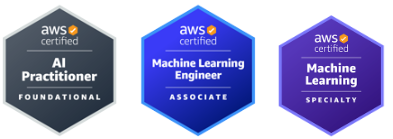
\includegraphics[width=0.6\linewidth]{genai.png}
            \end{figure}
        \end{onecolentry}
    
    
    \section{Summary}

    \begin{onecolentry}
        \begin{highlightsforbulletentries}


        \item 25+ years architecgtural experience in IT industry, with 8+ years in AI/ML, and 12+ years in cloud computing and hybrid infrastructure.
        
        \item Industries and domain knowledge in manufacturing, electronics, media, retails and public sectors
        
        \item  Curious, self-motivated, and a quick learner with strong problem-solving and hands-on skills

        \item  Effective communicator across stakeholders from CxO leadership to engineers, earn trust, build consensus and lead teams to deliver swift and impactful business results.
        
        \end{highlightsforbulletentries}
    \end{onecolentry}




    \section{GenAI Stack Skills}
        
        \begin{onecolentry}
            \textbf{AI Solutions:} Microsoft CoPilot/Agent/Studio, Github CoPilot, Amazon Q for Developer/Business/QuickSight, ChatGPT, Perplexity
        \end{onecolentry}

        \begin{onecolentry}
            \textbf{Managed AI/Agent Platforms:} AWS Bedrock/SageMaker, GCP Vertex AI, Azure AI, AnyScale, IBM WatsonX, NVidia AI Enterprise
        \end{onecolentry}

        \begin{onecolentry}
            \textbf{LLM Moodels:} GPT-4o/GPT-o1, Claude 3.5, Gemini 1.5, Llamda 3, Granite 3.0
        \end{onecolentry}

        \begin{onecolentry}
            \textbf{Managed Data Platforms:} Amazone Glue/Redshift/EMR, Databrick, Ray Data, Google BigQuery, IBM WatsonX Data
        \end{onecolentry}
        
        \begin{onecolentry}
            \textbf{Agent/DL/ML/Data OSS Frameworks/SDKs:} LlamaIndex, LangChain, Swarm, AutoGen, Ray, Hadoop, Spark, TensorFlow, PyTorch
        \end{onecolentry}       
        
        \begin{onecolentry}
            \textbf{Hybrid Infrastructure:} IoT, NVidia Jetson/ROS, Private Cloud, Hybrid Networking
        \end{onecolentry}        

        \begin{onecolentry}
            \textbf{Languages:} Python, Java, C\#, HTML/JS/TS/React/NextJS, Swift/Kotlin/Flutter, SQL
        \end{onecolentry}

    \section{Experience}
        
        \begin{twocolentry}{
            Septermber 2024 – Present
        }
            \textbf{Founder and CTO}, GenAI.Industries Consulting -- Chapel Hill, NC\end{twocolentry}

        \vspace{0.10 cm}
        \begin{onecolentry}
            \begin{highlights}
                \item GenAI and AI/ML expertise applied to industries and business problems
                \item Multi-cloud (AWS, Azure, GCP, IBM Cloud)  Architecture expertise to optimize IT and solution delivery 
            \end{highlights}
        \end{onecolentry}


        \vspace{0.2 cm}

        \begin{twocolentry}{
            January 2024 – August 2024
        }
            \textbf{Chief Systems Architect/Director}, Chamberlain Group -- Oak Brook, IL\end{twocolentry}

        \vspace{0.10 cm}
        \begin{onecolentry}
            \begin{highlights}
                \item Guided the overall architecture of the next-gen myQ system, supporting both residential and commercial platforms, including middleware, video platform, firmware, mobile apps, and system interfaces.
                \item Collaborated with architects, developers, and business stakeholders (Engineering, Product, IT, Marketing, QA, Operations, Customer Service) to translate product requirements into technical specifications, enhancing cross-departmental communication.
                \item Led the Github CoPilot adoption, Observability and AIOps initiatives
            \end{highlights}
        \end{onecolentry}

        \vspace{0.2 cm}

        \begin{twocolentry}{
            June 2023 – December 2023
        }
            \textbf{Director, Multicloud Architecture}, RCG Global Services -- Iselin, NJ\end{twocolentry}

        \vspace{0.10 cm}
        \begin{onecolentry}
            \begin{highlights}
                \item Define service offerings in multi-cloud, enterprise architecture and GenAI for large enterprise customers 
                \item Led strategic initiatives within the internal cloud community of practice, promoting cloud adoption and best practices
                \item Design and delivered initial LLM RAG and Agent PoCs 
            \end{highlights}
        \end{onecolentry}

        \vspace{0.10 cm}
        \begin{twocolentry}{
            November 2021 – June 2023
        }
            \textbf{Senior Solutions Architect}, AWS -- Chapel Hill, NC\end{twocolentry}

        \vspace{0.10 cm}
        \begin{onecolentry}
            \begin{highlights}
                \item Guided manufacturing, media, and public sector clients in architecting secure, resilient, and cost-effective cloud-native solutions using AWS best practices.
                \item Specialized in Cloud Foundation, Event-Driven Architecture, DevOps, and AI/ML
                \item Engaged with AWS industry product managers and engineering teams to influence new product direction and features co-developed with customers
            \end{highlights}
        \end{onecolentry}
        
        \begin{twocolentry}{
            Dec 2020 – November 2021
        }
            \textbf{Principle Dilvery Architect}, IBM Consulting Services-- Chapel Hill, NC\end{twocolentry}

        \vspace{0.10 cm}
        \begin{onecolentry}
            \begin{highlights}
                \item Provided overall technical leadership for a team of 80+ domain architects, software and ML engineers, DevOps, and QA engineers in delivering cloud-native, container-based solutions.
                \item Led the core DevOps team to enhance application reliability, performance, and security, optimizing resource utilization on Azure.
                \item Guided application teams to redesign and implement cloud-native design patterns and core frameworks, increasing deployment speed by 30\%.
            \end{highlights}
        \end{onecolentry}
        
        \begin{twocolentry}{
            July 2016 – December 2020
        }
            \textbf{Chief Technologist}, IBM Eletronics Industry GTM -- Chapel Hill, NC\end{twocolentry}

        \vspace{0.10 cm}
        \begin{onecolentry}
            \begin{highlights}
                \item GenAI and AI/ML expertise applied to industries and business problems
            \end{highlights}
        \end{onecolentry}        

        \begin{twocolentry}{
            December 2010 – July 2016
        }
            \textbf{Lead Sales Engineer}, IBM Hybrid Cloud - Retail and IoT Solutions -- Chapel Hill, NC\end{twocolentry}

        \vspace{0.10 cm}
        \begin{onecolentry}
            \begin{highlights}
                \item GenAI and AI/ML expertise applied to industries and business problems
            \end{highlights}
        \end{onecolentry}      
        
        \begin{twocolentry}{
            Nov 2020 – December 2010
        }
            \textbf{Senior Managing Consultant}, IBM WebSphere Consulting -- Chapel Hill, NC\end{twocolentry}

        \vspace{0.10 cm}
        \begin{onecolentry}
            \begin{highlights}
                \item GenAI and AI/ML expertise applied to industries and business problems
            \end{highlights}
        \end{onecolentry}      
        
        \begin{twocolentry}{
            May 1999 – November 2000
        }
            \textbf{Software Engineer}, CDI -- Chapel Hill, NC\end{twocolentry}

        \vspace{0.10 cm}
        \begin{onecolentry}
            \begin{highlights}
                \item GenAI and AI/ML expertise applied to industries and business problems
            \end{highlights}
        \end{onecolentry}             
   
    \section{Publications}
        
        \begin{onecolentry}
            \begin{highlights}
                \item \href{http://www.redbooks.ibm.com/abstracts/sg248101.html?Open}{SOA Policy, Service Gateway, and SLA Management - 2013}
                \item \href{https://www.oreilly.com/library/view/patterns-serial-and/0738498149/}{Patterns: Serial and Parallel Processes for Process Choreography and Workflow - 2004}
                \item \href{https://peterkovari.blog/wp-content/uploads/WebSphere-Application-Server-Enterprise-V5-and-Programming-Model-Extensions-sg246932.pdf}{WebSphere Application Server Enterprise V5 and Programming Model Extensions - 2003}
            \end{highlights}
        \end{onecolentry}


        \section{Certifications}
        
        \begin{onecolentry}
            \textbf{AWS Certified:} AI Practitioner, Machine Learning Engineer Associate, Machine Learning Specialty, Solutions Architect Associate, Solutions Architect Professional, SysOps Associate, Developer Associate, DevOps Engineer Professional, Data Analytics, Data Engineering 
        \end{onecolentry}

        \begin{onecolentry}
            \textbf{GCP Certified:} Associate Cloud Engineer, Professional Cloud Architect
        \end{onecolentry}

        \begin{onecolentry}
            \textbf{Azure Certified:} Azure Fundamentals
        \end{onecolentry}

        \begin{onecolentry}
            \textbf{IBM/Red Hat Certified:} Professional Cloud Architect, Openshift Container Platform Specialist, SOA Solution Designer-2007
        \end{onecolentry}

        \begin{onecolentry}
            \textbf{Open Group Certified:} TOGAF Enterprise Architect - 2010
        \end{onecolentry}

        \begin{onecolentry}
            \textbf{SUN Certified:} Java Programmer - 1999
        \end{onecolentry}        



        \section{Education}

        \begin{twocolentry}{
            June 1998 – Auguest 1999
        }
            \textbf{Binghamton University}, MS in Computer Science\end{twocolentry}
        \begin{twocolentry}{
                September 1991 – May 1996
            }
                \textbf{Beijing University}, BA in Foreign Language and Literature\end{twocolentry}           
        \vspace{0.10 cm}
        
        \begin{onecolentry}
            \begin{figure}
                \centering
                
\includegraphics[width=0.6\linewidth]{mc.png}
            \end{figure}
        \end{onecolentry}
    
\end{document}